\chapter{Zadanie 6.}
Dzia�anie algorytm�w przy zak��ceniu zmiennym sinusoidalnie wida� na rysunku ~\ref{dmc_zakl_sin}. Jest to zak��cenie bardzo trudne do wyr�wnania, st�d oba algorytmy nie nad��a�y z powrotem do warto�ci zadanej. Wida� jednak, �e uwzgl�dnienie zak��ce� w algorytmie spowodowa�o znaczn� popraw� regulacji - co prawda wykres wyj�cia jest dalej sinusoid�, jednak o wyra�nie ni�szej amplitudzie. �wiadczy to o tym, �e, w przypadku gdy obiekt jest nara�ony na zak��cenia, warto zastosowa� ten regulator zamiast klasycznego DMC.

\begin{figure}[b]
\centering
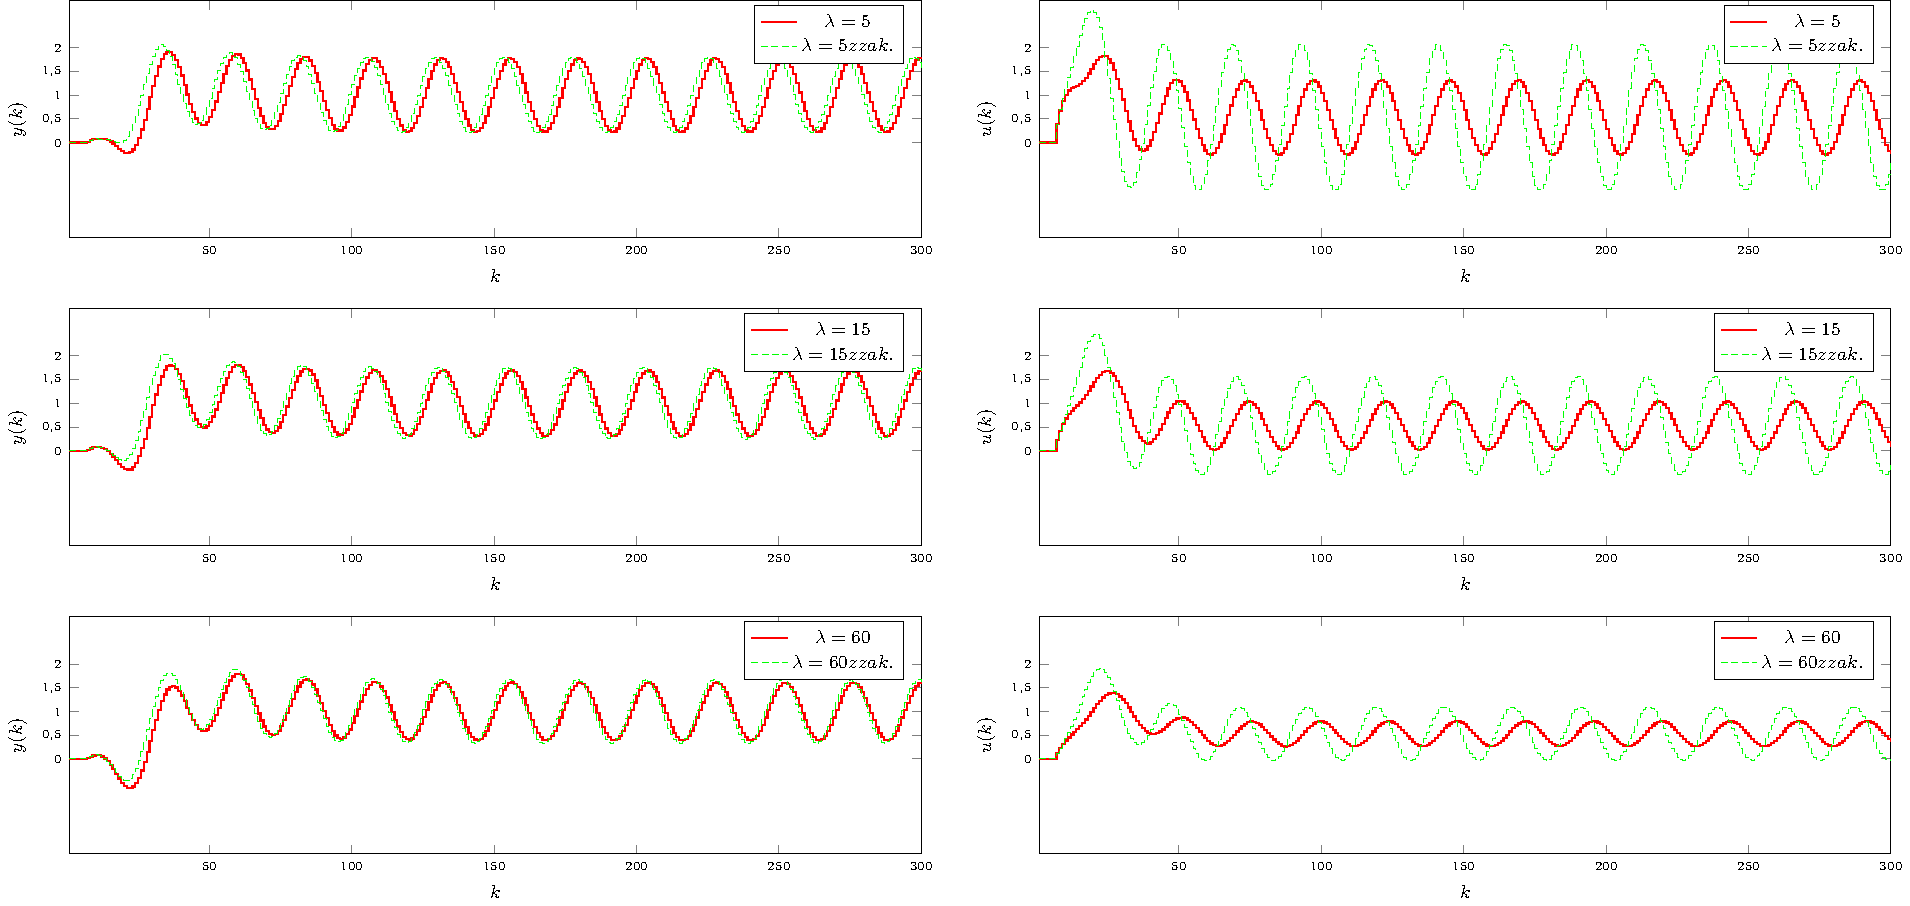
\includegraphics[scale=1]{../wykresy_pdf/zad6_dmc_zbiorczy.pdf}
\caption {Symulacja algorytmu DMC dla skoku zak��cenia}
\label{dmc_zakl_sin}
\end{figure}